\chapter{The fish population dynamics model}
\label{ch:model}

\section{Underlying equations}
\label{sec:underlying-equations}

The general model of SEAPODYM is based on a classical advection--diffusion--reaction (ADR) equation. Let $N(a,t,\mathbf{x})$ be the density of the fish population at age $a \in \left[0,\bar{a}\right]$, at time $t \in \left[t_0,t_{\text{fin}}\right]$ and at position $\mathbf{x}=(x,y) \in \Omega \in \mathbf{R}^2$. Herein for brevity we omit notations of age, time and space, and use the gradient operator $\nabla = (\partial_x, \partial_y)^{\text{T}}$ and the divergence operator of a two-dimensional vector field $\text{div}(\mathbf v)=\partial_x u+\partial_y v$.
\begin{linenomath}
The continuous version of SEAPODYM describing spatial, temporal and age dynamics of fish population density $N$ is represented by the system of ADR equations with an ageing term, the initial and boundary conditions:
\begin{align}
& \partial_t N+\partial_a N =-\text{div} (\mathbf{v} N ) +\nabla (D \nabla N) - M N \label{eq:model-1}\\
& N(a,\mathbf{x},t_0)  = N_0 (a,\mathbf{x})  \label{eq:model-2} \\
& N(0,\mathbf{x},t) =  S(t,\mathbf{x}) \label{eq:model-3}\\
& \mathbf n \cdot \mathbf v \Bigr\rvert_{\mathbf x \in \partial \Omega} = \mathbf n \cdot\nabla N \Bigr\rvert_{\mathbf x \in \partial \Omega} = 0 \label{eq:model-4}  
\end{align}
\end{linenomath}
where 
\begin{itemize}

\item[] $\mathbf{v}={\mathbf{v}}_c+{\mathbf{v}}_N$ is the velocity field including velocity of ocean currents ${\mathbf{v}}_c$ and directed movement velocities of population density ${\mathbf{v}}_N$ (see eqs.~\ref{eq:mean-currents} and \ref{eq:active-movement-velocity});
\item[] $D$ is the diffusivity (see eq.~\ref{eq:diffusion}); 
\item[] $M = m_N + m_F$ is the total mortality that is the sum of natural $m_N$ and fishing $m_F$ mortality rates (see eqs.~\ref{eq:Mvar} and \ref{eq:FM}); 
\item[] $N_0(a,\mathbf{x})$ in (eq.~\ref{eq:model-2}) is the initial value of the state vector, i.e. the population density for all ages $a \in \left[0,\bar{a}\right]$ in the two-dimensional space, where $\bar{a}$ is the maximal age of individuals in a given population; 
\item[] $S(t,\mathbf{x})$ in (eq.~\ref{eq:model-3}) gives the new recruited biomass after spawning, i.e. the boundary condition at $a=0$ (see eqs.~\ref{eq:larvae} and \hyperref[sec:reproduction]{\ref*{sec:reproduction}}); 
\item[] Neumann zero-flux boundary conditions (eq.~\ref{eq:model-4}) imply impenetrability of the two-dimensional domain $\Omega\in\mathbb{R}^2$ boundaries, $\partial \Omega$; 
and
\item[] $\mathbf{n}$ is the unit normal vector to $\partial\Omega$.
\end{itemize}


In addition to age dynamics, the model (\ref{eq:model-1}--\ref{eq:model-3}) describes the dynamics of four life stages. These are larvae, small juveniles, immature (young) and mature (adult) fish (Table \ref{tab:life_stages}). The reasoning behind considering these life stages is their different movement dynamics. Larvae drift in the surface where they are passively transported by ocean currents; hence their survival depends on the local environmental conditions in the sites to which they are transported. Small juveniles (for tunas, up to 3 months of age, for other fish species, age classes which cannot be considered autonomous in terms of movements) occupy the epipelagic layer, through which they start performing diel migrations to avoid predation. However, their large-scale horizontal movements are still passive and depend on currents in this layer. In the next life stage of young immature fish, in addition to being passively transported by ocean currents, fish can undertake directed movements in search of food. At the fourth life stage, mature adults, the fish have two drivers of movement -- survival, that is, searching for food, and reproduction, that is, moving to habitats that provide optimal conditions for spawning and for survival of larvae. Note that dynamics of all life stages are modelled by the general model (eqs.~\ref{eq:model-1}--\ref{eq:model-3}); however, the rates of reproduction, mortality and movement are considered differently. 


\begin{table}[!htb]
  \caption{
    Considered life stages of a modelled population. The column ``driver'' specifies the biological driver for active movement (both directed and non-directional).
  }
\centering
  \begin{tabular}{p{2.75cm}|p{2.25cm}|p{1.75cm}|p{3.5cm}|p{4cm}}
  \hline
%  \begin{tabular}{p{2.75cm}p{2.75cm}p{1.75cm}p{3.75cm}p{3cm}}
    \textbf{Life stage} & \textbf{Ages, $a$} & \textbf{Layer} & \textbf{movement} &\textbf{Driver}\\
    \hline   \hline
    Larvae         & $a=0$ & surface & passive drift & none\\
%    \hline
    Small juveniles& $0 < a \leq a_J$ & epipelagic & passive drift & none\\     
%    \hline
    Young adults   & $a_J <  a \leq a_Y$ & all & passive and active & survival \\   
%    \hline
    Mature adults  & $a_Y < a \leq \bar{a}$ & all & passive and active & survival, reproduction\\
    \hline%\hline
  \end{tabular}
\label{tab:life_stages}   
\end{table}

\section{Dynamic processes}
\label{sec:model-dyn}

SEAPODYM follows a biophysical approach explicitly describing the spatio-temporal dynamics of a species population density arising from animal behaviour as a response to environment. The environment is described by physical, biogeochemical and biological variables derived from external models. These variables are temperature, currents, dissolved oxygen, primary production, euphotic depth and density of micronektonic organisms that are the prey of tunas and other large predators (see section~\ref{sec:model-forcing}). As seen from the model (eqs.~\ref{eq:model-1}--\ref{eq:model-3}), the fish population dynamics in SEAPODYM are resolved in four dimensions: two-dimensional space, time and age. The vertical dimension is simplified into three pelagic layers. 

Two main drivers of animal behaviour, reproduction and survival, are considered. To integrate them into the model, two types of habitat indices, spawning $H_s$ and feeding $H_a$, are defined. Definitions of species habitats are based on empirical evidence. A thermal habitat of tuna species is derived from an individual heat budget model. The feeding habitat is computed according to the accessibility of tuna predator cohorts to the different vertically migrating and non-migrating micronekton (mid-trophic) functional groups. The spawning habitat is based on temperature and density of predators and food for larvae in the spawning sites. These habitats, as well as the movements, reproduction and survival, are driven by a biophysical environment predicted from a coupled ocean physical--biogeochemical model. 


\subsection{Species environment}\label{sec:model-forcing}

The species environment is described by the spatio-temporal fields of the following variables: i) physical -- temperature and ocean currents, ii) biochemical -- dissolved oxygen concentration, primary production and euphotic depth, and iii) biological -- the food resource for the species (see Table~\ref{forcing}). The temperature, dissolved oxygen concentration, and zonal/meridional currents are the three-dimensional outputs of coupled ocean general circulation (OGCM) and biogeochemical (BGCH) models. The euphotic depth and integrated primary production are the two-dimensional outputs of either BGCH models or observation-based empirical models. Three pelagic layers represent a simplified vertical dimension of SEAPODYM: the surface epipelagic layer, the subsurface mesopelagic layer and the deep mesopelagic layer. The current definition of these layers is based on the euphotic depth and originates from the definition of six functional groups of micronekton (Figure~\ref{fig:mnk_groups}). 


\begin{table}
\caption{Forcing variables used in SEAPODYM applications. The column {\bfseries Model} refers to the external model type. }
%\vspace{0.5cm}
\begin{tabular}{>{\bfseries}m{1.5cm}m{2.25cm}m{11.5cm}}
\hline
{Model} & {\textbf{Variables}} & {\textbf{ Description}}\\
\hline
\hline
\multicolumn{3}{c}{\cellcolor[gray]{0.8}\textit{Physical forcing}}\\
\footnotesize{OGCM} & $T$, $u,v$ &  Ocean reanalysis by general circulation model with atmospheric forcing based on meteorological observations. \\

\multicolumn{3}{c}{\cellcolor[gray]{0.8}\textit{Biogeochemical forcing}}\\

\footnotesize{BGCH} & $P$, $O_2$, $z_e$ & Primary production, dissolved oxygen and euphotic depth, either  predicted by BGCH model coupled to OGCM, or by empirical model (e.g. VGPM) derived from satellite data. \\


\multicolumn{3}{c}{\cellcolor[gray]{0.8}\textit{Biological forcing}}\\
\footnotesize{LMTL} & $F$, $Z$ & Six micronekton groups and one lower-trophic level group (zooplankton) predicted by SEAPODYM-LMTL model with the above forcing, excluding dissolved oxygen. \\
\hline
\label{forcing}
\end{tabular}
\end{table}

First, all three-dimensional environmental variables are averaged over three pelagic layers (Figure~\ref{fig:forcing_integration}). These integrated variables are then used to force the SEAPODYM-LMTL (Lower and Mid-Trophic Level) model. The SEAPODYM-LMTL model relies on primary production, temperature and ocean currents to simulate the biomass of six functional groups of micronekton, that is, mid-trophic-level prey organisms of tunas, residing or migrating through three pelagic layers within the upper 1000~m of the water column. The depth $\mathbf{z}$ of pelagic layers is linked to the depth of euphotic layer $z_e$ as follows: 
\begin{equation}\label{eq:pelagic-layers}
\mathbf{z}=(1.5 z_e,4.5 z_e,min(10 z_e,1000)). 
\end{equation}

\begin{figure}[H]
\centering
 \includegraphics[width=0.92\textwidth]{chapter1/figs/mnk-groups}
 \caption{The definition of micronekton functional groups by their vertical diel behaviour. }
 \label{fig:mnk_groups}
\end{figure}

\begin{figure}
 \centering
 \includegraphics[width=0.3\textwidth]{chapter1/figs/T-3d-grid}
 \includegraphics[width=0.3\textwidth]{chapter1/figs/T-3d-grid-zeu}
 \includegraphics[width=0.32\textwidth]{chapter1/figs/T-2d-grid}
 \caption{The integration of three-dimensional environmental variables. Here three-dimensional temperature (left) is integrated over three pelagic layers (middle) and divided by each layer's thickness to provide the two-dimensional mean fields of each forcing variable.}
 \label{fig:forcing_integration}
\end{figure}

The definition \eqref{eq:pelagic-layers} of pelagic layers in SEAPODYM is derived from the diurnal patterns in vertical distributions of micronektonic species shown by acoustic observations (see \citet{Lehodey2015} for further details on vertical layer definition and the SEAPODYM-LMTL model). The spatio-temporal fields of modelled micronekton together with the physical and biochemical variables are used to describe the preferred habitats of the large pelagics for foraging and spawning and to predict their temporal and spatial dynamics. 


Let us denote $var_{\mathbf{z}}(t,\mathbf{x})$, the forcing variable averaged over vertical layer $\mathbf{z}$, where $var$ can be either water temperature $T$, dissolved oxygen $O_2$, or ocean currents $u$ and $v$. As mentioned above, the primary production $P =P(t,\mathbf{x})$ is integrated through the whole water column (knowing that most of it is concentrated in the euphotic layer). Vertically integrated primary production is given in units of $\text{mmol C} \text{ m}^{-2} \text{d}^{-1}$. The density of micronekton $F_{z_d z_n}=F(t,\mathbf{x},z_{d},z_{n})$ refers to the modelled density of small nektonic organisms (representing prey of modelled predatory species) aggregated into a functional group by their vertical behaviour, that is, all inhabiting layer $z_d$ and $z_n$ during the day and night respectively, as shown in Figure~\ref{fig:mnk_groups}. For brevity, hereafter we omit dimensional notations (time, 2D space) for SEAPODYM forcing variables once they are defined. Also, for convenience let us represent all prey functional groups as a diagonal matrix of dimension $dim(\mathbf z) \times dim(\mathbf z)$,

\begin{equation}
 \mathbf{F} = \left( 
  \begin{array}{ccc}
	F_{11} & 0 & 0 \\
	F_{21} & F_{22} & 0 \\
	F_{31} & F_{32} & F_{33}
  \end{array} \right)
\label{eq:F}
\end{equation}

\noindent where the rows and columns show the composition of vertical layers during the day and night respectively.  

\subsection{Spawning habitat}\label{sec:spawning-habitat}
The spawning habitat describes the ensemble of environmental conditions that are favourable for spawning and optimal for larvae survival. In other words, the spawning habitat describes the ensemble of conditions that constrain larval production and mortality, and affect the subsequent recruitment. This habitat then represents the following four mechanisms:
\begin{itemize}
	\item changes in the spatial extent of the spawning habitat with temperature;
	\item coincidence of spawning with presence or absence of food for larvae (micro-zooplankton, approximated by primary production), that is, the match/mismatch mechanism proposed by Cushing (1975);
	\item coincidence of spawning with presence or absence of predators of larvae (that are the micronektonic organisms, i.e., the prey of adults); and
	\item redistribution of larvae by the oceanic circulation, which can retain larvae in favourable areas with lower natural mortality, or conversely move the larvae to unfavourable zones where the natural mortality will be higher. 
\end{itemize}

The favourability of tuna habitat in terms of spawning success and larvae survival depends on three oceanic variables -- sea surface temperature ($SST(t,\mathbf{x})$), prey of larvae ($\Lambda(t,\mathbf{x})$, can be either plankton density or primary production as a proxy), and density of predators of larvae present in the surface layer, which are also the food for spawners ($F_1(t,\mathbf{x})$, surface micronekton, see below).  

The index of spawning habitat, $H_s(t,\mathbf{x}) \in (0,1)$, is defined as the following product (for brevity, we omit here the dimensional notations of environmental variables, micronekton density and habitats):

\begin{align}
	H_s = f_1(SST;{T}^{*},\sigma) \times f_2(\Lambda,\alpha) \times f_3(F_1,\alpha_F,\beta_F),
\label{eq:spawning_habitat}
\end{align}

\noindent requiring that all three environmental conditions are optimal for the species for the habitat index to be maximal. These three functions (see Figure~\ref{fig:reproduction-funcs}) are defined between 0 and 1 as follows. The thermal conditions are described by

\begin{equation}
f_1 = e^{-\frac{\left(SST-T^*\right)^2}{2\sigma^2}},
\label{eq:spawning-thermal}
\end{equation}

\noindent a Gaussian function with two parameters, ${T}^{*}$ and $\sigma$, being the optimal temperature and thermal tolerance interval of larvae respectively. The function $f_2$ is the analogue of the Holling type III functional response function with $n=2$:

\begin{equation}
f_2=\frac{\Lambda^n}{\alpha+h\Lambda^n},
\label{eq:spawning-prey}
\end{equation}

\noindent where handling time $h=1$ (to allow the function scaling within $[0,1)$ interval) and $\alpha\ge0$ the inverse of searching efficiency defining the shape of functional response to the prey densities (no response with $\alpha=0$, mostly hyperbolic within the effective range of prey densities as the inflection point $\Lambda=\sqrt{\frac{\alpha}{3}}$ gets too close to 0 with small $\alpha$ and marked logistic relationship with large enough $\alpha$). Note that when using primary production $P$ as a proxy for the density of phyto- and zooplankton, which are the actual prey of larvae, we should convert primary production to the wet weight of plankton. So if ocean primary production $P$ is given in mmol$\cdot$C$\cdot$m$^{-2}$, we use the energy transfer constant $E=0.354$ to compute the part of $P$ that will be transferred to lower-trophic level groups \citep*[see][]{Lehodey2015} and the conversion factor $c=0.1415$~gWW$\cdot$mmol$^{-1}$~C \citep{Iverson}, so that $\Lambda=cEPt$, the $t$ being the unit time of production $P$, provides the wet weight of plankton species in the units of g$\cdot$m$^{-2}$. 


The third function, $f_3$, is the log-normal distribution function rescaled on $(0,1)$ allowing selection of the optimal window of micronekton densities $F_1$ in the surface layer:

\begin{equation}
f_3 = \frac{1}{F_1 e^{0.5\beta^2_F-\alpha_F}} e^{-\frac{\left(\log{F_1}-{\alpha_F}\right)^2}{2\beta^2_F}}
\label{eq:spawning-pred}
\end{equation}

\noindent where parameters $\alpha_F$ and $\beta_F$ are the mean and standard deviation of log-normal distribution function, and the surface micronekton densities $F_1$ (1 is the layer index) is computed as follows: 

\begin{equation}
F_1 = \tau {\mathbf F_{1 \cdot}}{\mathbf \delta} +(1-\tau) {\mathbf {F_{\cdot 1}}^{\mathsf{T}}} {\mathbf \delta}
\label{eq:pred-surface}
\end{equation}

\noindent with $\mathbf{\delta}=(1,1,1)^{\mathsf{T}}$ and $\tau$ is the proportion of light hours in a 24-hour cycle. In other words, $F_1$ is the density of all micronektonic organisms present in the epipelagic layer during the day, ${\mathbf F_{1 \cdot}}$, and during the night, ${\mathbf {F_{\cdot 1}}^{\mathsf{T}}}$, either residing or migrating here from deeper layers. However, larvae predation is likely maximal during daytime and twilight periods, and therefore only two twilight hours are considered in the second term; hence the formula~\ref{eq:pred-surface} simplifies to 

\begin{equation}
F_1 = \tau {\mathbf F_{1 \cdot}}{\mathbf \delta} + {\mathbf {F_{\cdot 1}}^{\mathsf{T}}} {\mathbf \delta}/12
\label{eq:pred-surface2}
\end{equation}

%the density of predators of larvae ~\ref{eq:pred-surface} is computed as the sum of mid-trophic biomass in the epipelagic layer during daytime (the daylength) and epi- and migrants from deeper pelagic mid-trophic biomass during the sunrise and sunset hours only. In practice, in model applications

\subsection{Reproduction}\label{sec:reproduction}
Successful larval recruitment is linked to both the spawning stock density and the conditions of larvae survival. Hence, the number of recruited larvae $N(0,t,\mathbf{x})$ is the product of $H_s$ (eq.~\ref{eq:spawning_habitat})  and the stock-recruitment function of density of mature adults.

The total amount of  mature adults in each position of two-dimensional space, $\hat{N}(t,\mathbf{x})$, is computed using the continuous maturity function $\mu=\mu(a)$ obtained from external studies (see section~\ref{sec:sp-biology}) and the density of adult tuna predicted by the model (for brevity, hereafter we leave notation of age dimension and deliberately omit (time, 2D space) notations for SEAPODYM state variables):
\begin{equation}
	\hat{N} = \int_{a_J}^{\bar{a}}{\mu(a)N(a)da}
\label{eq:Nmature}
\end{equation}

\noindent where $a_J$ is the last age in a small juvenile stage and $\bar{a}$ is the maximal age of individuals in the population. The number of new recruits at zero age, $N(0,t,\mathbf{x})$, that is, the term $S$ in eq.~\ref{eq:model-1}, is then the product of the Beverton--Holt stock-recruitment function \citep{Beverton-Holt} and the spawning habitat index:

\begin{equation}
	N(0) = H_s \frac{r\hat{N}}{1+b\hat{N}}
\label{eq:larvae}	
\end{equation}	

\noindent where $r$ is the reproduction rate and $b$ is a parameter defining the strength of the stock--recruitment relationship between the density of spawners, $\hat{N}$ (in $\text{Nb}\cdot\text{km}^{-2}$, Nb - number of individuals), and those of larvae, $N(0)$, survived and recruited to the first age class (Figure~\ref{fig:reproduction-funcs}). This relationship is suitable for opportunistic spawners, for which the spawning success depends on the local spawning habitat index and the adult biomass.   

\begin{figure}
 \centering
 \includegraphics[width=0.92\textwidth]{chapter1/figs/reproduction-funcs}
 \caption{Functions used in the definition of spawning habitat and reproduction: (a) Beverton--Holt stock--recruitment function, (b)thermal function $f_1$, (c) prey function $f_2$, and (d) predator function $f_3$, based on parameters estimated for bigeye tuna \citep{Senina2020b}.}
 \label{fig:reproduction-funcs}
\end{figure}

\subsection{Growth and maturity}\label{sec:sp-biology}

SEAPODYM uses the species' biological parameters estimated in external studies, which are usually obtained from fitting the classical \citet{Bertalanffy} growth equation either to data derived either from conventional tagging or from otolith increments. This equation assumes that as the organism ages, its length increases to an asymptote $\ell_{\infty}$, which is the greatest possible length that the organism can attain under the given conditions:

\begin{equation}
\ell(a) = \ell_{\infty}\left(1- \mathrm{e}^{(-k(a-a_0)}\right)
\label{eq:vonBertalanffy}
\end{equation}

\noindent where $\ell(a)$ is length of a species at age $a$, constant $\ell_{\infty}$ is asymptotic length corresponding to the known maximum length of the oldest fish, $k$ is growth rate, and $a_0$ is age ``zero'' length. In SEAPODYM, the relationships length-at-age and its inverse are used in the definitions of habitats, the integration of length frequency and tagging data.

%\citep{Beverton-Holt} (Huxley, 1924):
The weight of organisms relates to length-at-age following the general allometric relationship:

\begin{equation}
w(a)=q{\ell}(a)^p
\label{eq:weight-at-length}
\end{equation}

\noindent with the power constant $p$ estimated by fisheries biologists from weight and length measurements. For many fish and tuna species, the constant $p \approx 3$, meaning that the coefficient $q$ is the fraction of the volume of a cube of side $\ell$ that the organism occupies \citep*[see][]{Beverton-Holt}. The species' weight-at-age function has the asymmetrical sigmoid form and is used in SEAPODYM to compute the species' thermal inertia (section~\ref{sec:accessibility}) and in predicting catch statistics (section~\ref{sec:predicted-catch}).

\vspace{0.1cm}
Maturity-at-age is another external (fixed) parameter in SEAPODYM. Two ways of defining maturity in the model are proposed: 
\vspace{-0.1cm}
\begin{itemize}
\item[(i)] ``knife-edge'' maturity, occurring from immature to the mature state at age when $50\%$ of individuals are mature, $a_{50}$, so that only adults older than age $a_{50}$ (equivalent to $a_{Y+1}$ in Table~\ref{tab:life_stages}) are considered capable of reproducing. This means that in the equation~\ref{eq:Nmature} of spawning stock biomass, maturity $\mu(a)=0$ for all $a<a_{50}$ and $\mu(a)=1$, otherwise;
\item[(ii)] the continuous maturity function $\mu(a)$, giving the estimation of maturity at age expressed in values between 0 and 1 equal to the portion of mature adults at a given age $a$. In this case the continuous function is used in eq.~\ref{eq:Nmature}. 
\end{itemize}


\subsection{Feeding habitat and movement rates}

The quality of feeding habitat controls the directed component of tuna density movement. We define the \textbf{index of feeding habitat as the micronekton density that is accessible to the predator}. This index is therefore not null when the predators and prey share the same habitats and the environmental conditions in the prey's habitat can be tolerated by the predator. 

\subsubsection{Accessibility}\label{sec:accessibility}

\begin{figure}%[htbp]
	\centering
        \includegraphics[width=0.85\textwidth]{chapter1/figs/thermal-preference}
	\caption{Changes in thermal preferences function $f_4$ linked to species' growth: the optimal temperature decreases with increased body size, while standard deviation increases with increased body weight. Two panels depict examples of typical parametrisation for (a) skipjack and (b) bigeye tuna.}
	\label{fig:thermal-preference}
\end{figure}


The accessibility of a species to a pelagic layer depends on environmental conditions and the species' preferences and/or tolerances related to these conditions, which vary with age (size). In SEAPODYM, we consider species' thermal preferences and oxygen demands as two main factors stipulating species' accessibility to a given depth and position in two-dimensional space, $\Theta(a,t,\mathbf{x},z)$. For brevity, hereafter we leave notation of age dimension and deliberately omit (time, space) notations for SEAPODYM variables depending on environment once they are defined. Thus, accessibility $\Theta(a)$ to a given vertical layer is the product of the two functions -- temperature and oxygen in the corresponding layer:

\begin{align}
&\Theta(a) = f_4(T;{T}^{*}(a),\sigma(a)) \times f_5(O_2;O_2^{*},\gamma)
\label{eq:accessibility}
\end{align}

\noindent where $f_4$ is the Gaussian function selecting the interval of preferred temperatures around the optimal value ${T}^{*}(a)$ and the width of the interval depending on $\sigma(a)$ (Figure~\ref{fig:thermal-preference}):

\begin{equation}
  \label{eq:feeding-thermal}
  f_4 = \mathrm{e}^{\left(-\dfrac{( T - {T}^{*}(a))^2}{2 \sigma^2(a)}\right)}
\end{equation}

\noindent It is known that species have different tolerances to oxygen levels. The lowering of oxygen concentration can quickly make the habitat unfavourable for tunas, expressed in behavioural responses such as increased speeds \citep*[see, e.g.][]{Brill}. The effect of oxygen on the habitat quality can be described by a sigmoid function, $f_5$, stipulating the minimal level of dissolved oxygen necessary for the modelled species (Figure~\ref{fig:oxygen-tolerance}), with the response to near-critical values of oxygen defined by the parameter $\gamma$:

\begin{equation}
  \label{eq:oxygen}
  f_5=\frac{1}{1+\gamma^{(O_2-O_2^{*})}}
\end{equation}


\begin{figure}%[htbp]
	\centering
        \includegraphics[width=0.65\textwidth]{chapter1/figs/fig-oxyfuncs}
	\caption{Dependence of feeding habitat on oxygen level. Parameters for skipjack and bigeye tunas were obtained with help of MLE method using catch, catch at size and tagging data in the likelihood and objectively analysed oxygen climatologies from World Ocean Atlas \citep{Senina2018, Senina2021}.}
	\label{fig:oxygen-tolerance}
\end{figure}

\subsubsection{Age dependence}\label{sec:age-dependence}

The use of a Gaussian distribution with a preferred temperature mean linked to the fish size-dependent body temperature at steady state, and with a standard error of the distribution linked to the thermal inertia of the fish was formulated in \citet{Lehodey2003} based on earlier works on heat budget models \citep{Holland,Brill,Maury}. It is assumed that for a given species there is an \textit{optimal intrinsic temperature} ($T^{*}$) that remains constant whatever the age/size, and that this temperature is a target temperature for any individual of the species (e.g., due to genetic and physiological adaptation during species evolution). As demonstrated by a tuna heat budget model \citep{Holland}, when becoming larger with age, the fish will have to search for a colder habitat to compensate for their increasing body temperature at steady state. But they will also have a larger temperature range due to their thermal inertia increasing with size $\ell(a)$. Therefore we define the population \textbf{size-dependent thermal preference} with optimal temperature decreasing with size and tolerance interval linearly increasing with weight (Figures~\ref{fig:thermal-preference}, \ref{fig:mean-temperature}).

\begin{figure}[htbp]
	\centering
        \includegraphics[width=0.65\textwidth]{chapter1/figs/mean_temperature}
	\caption{Habitat temperature computed as a weighted spatio-temporal mean, with weights being the population density $N(a,t,\mathbf{x})$. Temperature profiles were obtained by means of parameter estimation for skipjack tuna using different datasets and experimental configurations \citep*[see][for more details]{Senina2016}.}
	\label{fig:mean-temperature}
\end{figure}

Let each age $a$ have corresponding fork-length $\ell(a)$ (eq.~\ref{eq:vonBertalanffy}) and weight $w(a)$ (eq.~\ref{eq:weight-at-length}). Thermal preference implies that the maximal average temperature occurs at age 0, that is, spawning (Figure~\ref{fig:mean-temperature}). We  assume   that  the   species   intrinsic  temperature  $T^{*}=T_0$ is equivalent to  the temperature preferred by the individuals at $a=0$. Then that thermal preference component of the accessibility function has parameters that are functions of age (through dependence on size) as follows:

\begin{align}
  {T}^{*}(a) = T_0-(T_0-T_m){\left(\frac{\ell(a)}{\ell(A^{+})}\right)}^{b_T},
\label{eq:temperature-length}
\end{align} 

\begin{align}
  \sigma(a) = \sigma_0+(\sigma_m-\sigma_0)\frac{w(a)}{w(A^{+})},
\label{eq:sigma-weight}
\end{align} 

\noindent where $T_0$, $T_m$ are the model parameters, denoting temperatures preferred by fish at age 0 and at maximal age ($A^{+}$), and $\sigma_0$, $\sigma_m$ are standard deviations in Gaussian thermal functions (eq.~\ref{eq:feeding-thermal}) for youngest and oldest cohort respectively. The parameter $b\in(1,p)$ allows the linear to approximately cubic ($p \approx 3$ in eq.~\ref{eq:weight-at-length}) relationship between preferred temperature and fish size, with $b=1$ equivalent to a linear decrease with species length at age, $\ell(a)$, and with $b=p$ equivalent to a linear decrease with species weight at age, $w(a)$. Note that, according to the heat budget model outcomes, we may assume that $\sigma_0=\sigma$ and $T_0=T^*$ in the spawning habitat definition (eq.~\ref{eq:spawning-thermal}), that is, that the species' preferred range and the optimal intrinsic temperature are the same as the range and the optimal temperature at larval stage. However, due to the use of integrated temperature fields (Fig~\ref{fig:forcing_integration}), the estimated optimal temperature for spawning might not correspond to the actual temperature at age ``0'' that the fish are seeking. For this reason, these parameters may be considered separately.


\subsubsection{Feeding habitat index}\label{sec:feeding-habitat}

The index of feeding habitat $H_a \in (0,1)$ is a linear combination of the abundance of the  six functional groups of micronekton inhabiting three pelagic layers (eq.~\ref{eq:F}), with the coefficients being the accessibilities to the corresponding pelagic layer (see Table~\ref{tab:forage-in-layers}). However, the biomass levels of micronekton should be considered with caution due to uncertainty associated with the calibration of energy transfer coefficients, which control the total abundance of each functional group \citep{Delpech}, and the lack of information to derive the vertical distribution of the biomass from acoustic data \citep{Lehodey2015}. Therefore, one parameter, $E_{ij}$, per functional group has been added to account for an uncertainty on the absolute value of micronekton biomass density as well as to include the possible effect of food preference of the predator species. Then the matrix $\mathbf{F}$ can be rewritten as:

\begin{equation}
 \mathbf{F} = \left( 
  \begin{array}{ccc}
	E_{11}\cdot F_{11} & 0 & 0 \\
	E_{21}\cdot F_{21} & E_{22}\cdot F_{22} & 0 \\
	E_{31}\cdot F_{31} & E_{32}\cdot F_{32} & E_{33}\cdot F_{33}
  \end{array} \right).
\label{eq:eF-matrix}
\end{equation}

Finally, knowing the accessibility of the predator at age $a$ to each vertical layer $z$ with prey species, $\boldsymbol{\Theta}(a,z)$, which is the row vector of size 3 (number of vertical layers) at each $t$ and position $\mathbf{x}$ , the feeding habitat at age, at each spatial position and model time step can be written as follows:

\begin{equation}
	H_a(a) = \boldsymbol{\Theta}(a) \times \left(\tau {\mathbf F}{\mathbf \delta} +(1-\tau) {\mathbf F^{\mathsf{T}}} {\mathbf \delta}\right),
\label{eq:Ha}	
\end{equation}

\noindent where ${\mathbf F}$ is the matrix~\eqref{eq:eF-matrix}, $\mathbf{\delta}=(1,1,1)^{\mathsf{T}}$, and the weights $\tau$ denote the duration (portion) of daytime to account only for the micronekton biomass when it is present in the layer accessible by the predator. Note that the vector product in eq~\ref{eq:Ha}, $H_a(a,t,\mathbf{x})$, is a scalar field of a unitless quantity. The coefficients $E$, besides modifying the vertical structure of micronekton groups (although preserving their original two-dimensional distributions predicted by the SEAPODYM-LMTL model), have an important physical meaning, that is the inverse of the maximal (asymptotic) value of the density of a given micronekton group, in order to consider the feeding habitat attractive to the predator. The latter theoretically provides that each term of the linear combination~\eqref{eq:Ha} is limited within the $(0,1)$ interval. Besides, due to the Gaussian form of the thermal accessibility function and the definition of vertical layers, two layers cannot be favourable to a species at a given age and point in space and time. So, in practice the habitat index is either the sum of nearly zero contributions of micronekton groups if the conditions in neither layer are favourable, or the selection of micronekton biomass (scaled) in the preferred layer. To ensure in practice that the condition on the resulting index $H_a\leq1$ is met everywhere and for all age classes, additional scaling using a continuous rotated hyperbola function is applied throughout the model dimensions to reset to 1 all $H_a>1$ values obtained from the formula \eqref{eq:Ha}. Since the calibration of parameters $E$ is done by means of constrained function minimisation (Chapter~\ref{ch:parametrisation}), the final habitat is nudged to vary between 0 and 1, and the habitat gradient to provide local cues for predator movements (see section~{\hypersetup{linkcolor=black}{\bfseries \nameref{sec:movement}}} below). 

\subsubsection{Passive movement}\label{sec:oceanic-currents}
We denote $\mathbf{v}_z(t,\mathbf{x})$ the mean horizontal ocean current velocity at time $t$ and position $\mathbf{x}$, averaged over vertical layer $z$. The model simulates passive transport of tuna larvae and small juveniles. Densities of these life stages are transported by oceanic currents in the surface (epipelagic) layer, so the total velocity in~\ref{eq:model-1}, $\mathbf{v}=\mathbf{v}_0$ for ages $[0,a_J]$. Note that for most tuna species the movement dynamics at early life stages is changing rapidly with fish growth. Thus, tuna larvae occupy the upper 50~m of water column \citep{Llopiz}, while small juveniles are capable of diel migrations through the euphotic layer. Hence it is more realistic to use the near-surface currents  to describe the transport of fish at the larval stage and the currents integrated over the epipelagic layer to model advection of small juveniles. More accurate representation of vertical distribution of these early life stages will allow a more realistic description of their horizontal drift.

Whatever the size of the fish, the horizontal oceanic currents influence the movement of fish living in the water column. To incorporate the drift that the fish may experience while performing vertical diel migrations through layers $z$, we calculated the integrated current velocity through the water column, accounting for the time fish spend in each layer during the day and night. This time can be assessed as relative feeding habitat index, that is, for each $t$ and $\mathbf{x}$ we first compute the habitat component in each layer as:

\begin{equation}
 H_a(a,z) = \Theta(a,z) \left( \tau \mathbf{F}_{z \cdot} \mathbf{\delta} +(1-\tau) \mathbf{F}_{\cdot z}\mathbf{\delta}\right)
\end{equation}

\noindent where $\mathbf{F}$ is matrix~\eqref{eq:eF-matrix}. Then the time spent in each layer can be approximated by the relative contribution of the accessible micronekton density to the total accessible micronekton: 

\begin{equation}
 \label{eq:relative-habitat}
 \vartheta(a,z)=\dfrac{H_a(a,z)}{\epsilon+\displaystyle\sum_{z=0}^{z=2} H_a(a,z)}
\end{equation}
  
\noindent where the small constant $\epsilon$ is added to avoid division by zero. Then the averaged velocity, weighted by the time spent in the layer is computed as:

\begin{equation}
    \label{eq:mean-currents}
      \tilde{\mathbf{v}}_c(a) = \sum_{z=0}^{z=2}\vartheta(a,z) \mathbf{v}_z,
%      \tilde{\mathbf{v}}_c(a) = \mathbf{\vartheta}(a) \times \mathbf{v}_c,
 \end{equation}
 
\noindent with $\mathbf{\vartheta}(a)$ and the total velocity in~\eqref{eq:model-1} is

\begin{equation}
  \label{eq:mean-currents-ages}
  \mathbf{v}_c(a) =\left\lbrace
  \begin{array}{llll}
    \mathbf{v}_0   &\mbox{if}& a\leq a_J & \mbox{larvae and juveniles}\\
    \tilde{\mathbf{v}}_c(a) &\mbox{if}& a>a_J & \mbox{adults}
  \end{array}
  \right.
\end{equation}


\subsubsection{Active directed movement}\label{sec:movement}
The movement dynamics in SEAPODYM are governed by the advection--diffusion terms in model~\eqref{eq:model-1}. Thus, directed movements are modelled with the advection component of the model equation, while random (non-directional) dispersal is described by diffusion. Similar to Lagrangian models of individual behaviour, the movements of population density in a Eulerian approach are stipulated by local conditions only. Repeated responses to local cues at the individual level result in movements towards more favourable parts of the environment. These processes are formulated within Eulerian models by allowing the velocity field of population density to be proportional to the gradient of the movement stimuli. Hence, the velocity of directed movements of fish density, $\mathbf{v}$, is proportional to the gradient of the vector field of movement stimuli $\mathbf{I}$: 

\begin{equation}
\label{eq:density-velocity}
\mathbf{v}=\chi \nabla \mathbf{I}
\end{equation}

\noindent with the coefficient of proportionality, the so-called taxis coefficient, $\chi$.  

For any type of movements, the displacement per unit of time is directly dependent on the size of the individuals. Since the SEAPODYM-MASS model resolves population dynamics in age, we can easily formulate the movement rates at age. The movement stimuli are the feeding resource's densities becoming increasingly accessible to fish as they grow, which is described by the feeding habitat index \eqref{eq:Ha}. However, it is also known that the maximal sustainable speed of an individual is linked to its size through physiological mechanisms and not only because of variable environment \citep*[see e.g.,][]{Cayre, Brill, Nihira, Turchin}. To account for this we introduce a link between the density velocity field and the maximal sustainable speed at age (size) by making the coefficient of proportionality in the classical approach~\eqref{eq:density-velocity} a function of age, $\chi(a)$. So the directed component of density velocity field at time $t$ and in position $\mathbf{x}$ is proportional to the gradient of feeding habitat as follows:  

\begin{align}
	\mathbf v_N(a) = \chi(a)\left(\frac{\partial H_{a}}{\partial x}, \frac{\partial H_{a}}{\partial y}\right)^{\text{T}},
\label{eq:active-movement-velocity}	
\end{align}

\noindent where $\chi(a)\propto V_{max,a}$, with the maximal sustainable speed, $V_{max,a}$, being the maximal speed of a population density, hence the mean speed of a large number of individuals. It is linked to the mean individual size at age through the allometric relationship $V_{max,a}=V\ell_a^A$, with parameters $V$ expressed in body length per second ($BL/s$) and the power constant $A<1$ allowing a decrease of the speeds in $BL\cdot s^{-1}$ with increasing size. Note, to ensure that the resulting speeds from~\eqref{eq:active-movement-velocity} do not exceed the $V_{max,a}$, it is necessary that the norm of the velocity $\|\mathbf{v}_N(a)\|=V_{max,a}$ at highest habitat gradients. Thus, denoting $g_{m}=\text{max}(\|\nabla H_a\|)$, \footnote{Note that in the current version of code a simplified formula is implemented for a special case when $\Delta x = \Delta y$.} we may formulate the taxis coefficient as 

\begin{equation}
\chi(a)=g^{-1}_{m} V \ell_a^A 
\label{eq:taxis-coefficient}
\end{equation}

\noindent with parameters $V$ and $A$ the control parameters to be estimated with the help of the MLE approach (see Figure~\ref{fig:mean-movement}),  for example, informing them from movement data, such as conventional tagging (more details about the method in Chapter~{\hypersetup{linkcolor=black}{\bfseries \nameref{ch:parametrisation}}}, section~\ref{sec:model-tags}).

\subsubsection{Active random movement}\label{sec:directed-movements}

The diffusion term in model~\eqref{eq:model-1} describes random non-directional movements of a large number of individuals. Such movements are made by individuals when there is no preferred direction for movement, or when the local conditions became unfavourable (e.g., no more food). Besides, we can expect that individuals stay longer in the presence of favourable conditions (hence low diffusion), but will want to escape quickly from unfavourable habitats (high diffusion). Diffusion rate, or diffusivity, $D$ in \eqref{eq:model-1}, is therefore also linked to the feeding habitat index $H_a$, allowing an increase of non-directional movement velocities in a very poor habitat and minimising random displacements within a favourable habitat. Such a link is formulated as follows for each age $a$, at time $t$ and position $\mathbf{x}$:

\begin{align}
	D(a) = \sigma D_0 \left( 1-c{H^p_a}(a)\right) 
\label{eq:diffusion}	
\end{align}

\noindent where $\sigma$ is a constant parameter, the coefficient $D_0$ is the mean theoretical diffusion rate in an unfavourable (zero) habitat, parameter $c$ controls the reduction of $D_0$ with increasing habitat index; the constant $p=3$ is chosen to limit the reduction of $D_0$ in the lowest habitat indices $H_a<0.5$, making diffusivity less sensitive (always highest) in the poor quality habitat and rapidly increasing in the favourable habitat. 

The coefficient $D_0$ is derived from the theoretical formula for two-dimensional mean square displacement $r^2=4Dt$. Thus, if we make the assumption, although unrealistic, that at zero habitat all individuals move at their maximal speed $\bar{V}$ without turning, that is, mean square displacement at the time interval $\Delta T$ can be expressed as $r^2=\frac{1}{n}\sum\limits^n_{i=1}{(V_i \Delta T)^2}={\bar{V}}^2 {\Delta T}^2$, then we may compute the maximal theoretical diffusivity as

\begin{equation}
D_0=\frac{{\bar{V}}^2 \Delta T}{4},
\label{eq:theoretical-diffusivity}
\end{equation}

\noindent where the average speed of fish is assumed to be $\bar{V}=1~BL \cdot s^{-1}$ for any $a$. Since this formula obviously overestimates the diffusivity due to the unrealistic assumption above, we add the proportionality constant $\sigma$, the meaning of which is the reduction of the maximal theoretical diffusivity \eqref{eq:theoretical-diffusivity}. Note that~\eqref{eq:theoretical-diffusivity} models the non-linear increase of diffusivity with age (see Figure~\ref{fig:mean-movement}).

\begin{figure}[htbp]
  \centering
  \includegraphics[width=0.74\textwidth]{chapter1/figs/mean_movement_rates}
  \caption{Mean movement rates estimated for skipjack tuna using different datasets and experimental configurations: (top) directed velocity of population density in body length per second units at age; (bottom) average diffusion rates at age. The movement rates were averaged over space and time, with weights being spatio-temporal distributions of density $N(a,t,\mathbf{x})$ \citep*[see][for more details]{Senina2016}.}
  \label{fig:mean-movement}
\end{figure}

\subsubsection{Seasonal spawning migrations}\label{sec:seasonal-migrations}
One of the hypotheses of how the search of spawning grounds occurs assumes that adult tuna tend to direct their movements to find a place with environmental conditions like those occurring during their birth \citep*[see e.g.,][]{Cury}. Another hypothesis, which is used in SEAPODYM modelling, implies that the change in daylight triggers the switch from foraging to spawning behaviour \citep{Lehodey2008}. These two hypotheses can be implemented as follows. At every time $t$ and latitude $y$, a continuous seasonal switch function $\varsigma(t,y)$ enables rapid switching between two habitats depending on the function of daylight, so that the habitat of mature adults can be computed as a linear combination of feeding and spawning habitats:

\begin{equation}
  H = \varsigma H_a+(1-\varsigma) H_s	
\label{eq:seasonal-habitat}
\end{equation}

\noindent where the switch $\varsigma(t,y)$ is a step function defined as follows:

\begin{equation}
\varsigma(t,y)=\left(1+\alpha^{\varrho-\varrho_s} \right)^{-1} 
\label{eq:switch-function}
\end{equation}

\noindent with constant $\alpha$ defining the abruptness of the switch, $\varrho(t,y)$ is a function of a day length and $\varrho_s$ is the critical value that triggers the switch. 

\begin{figure}[htbp]
  \centering
  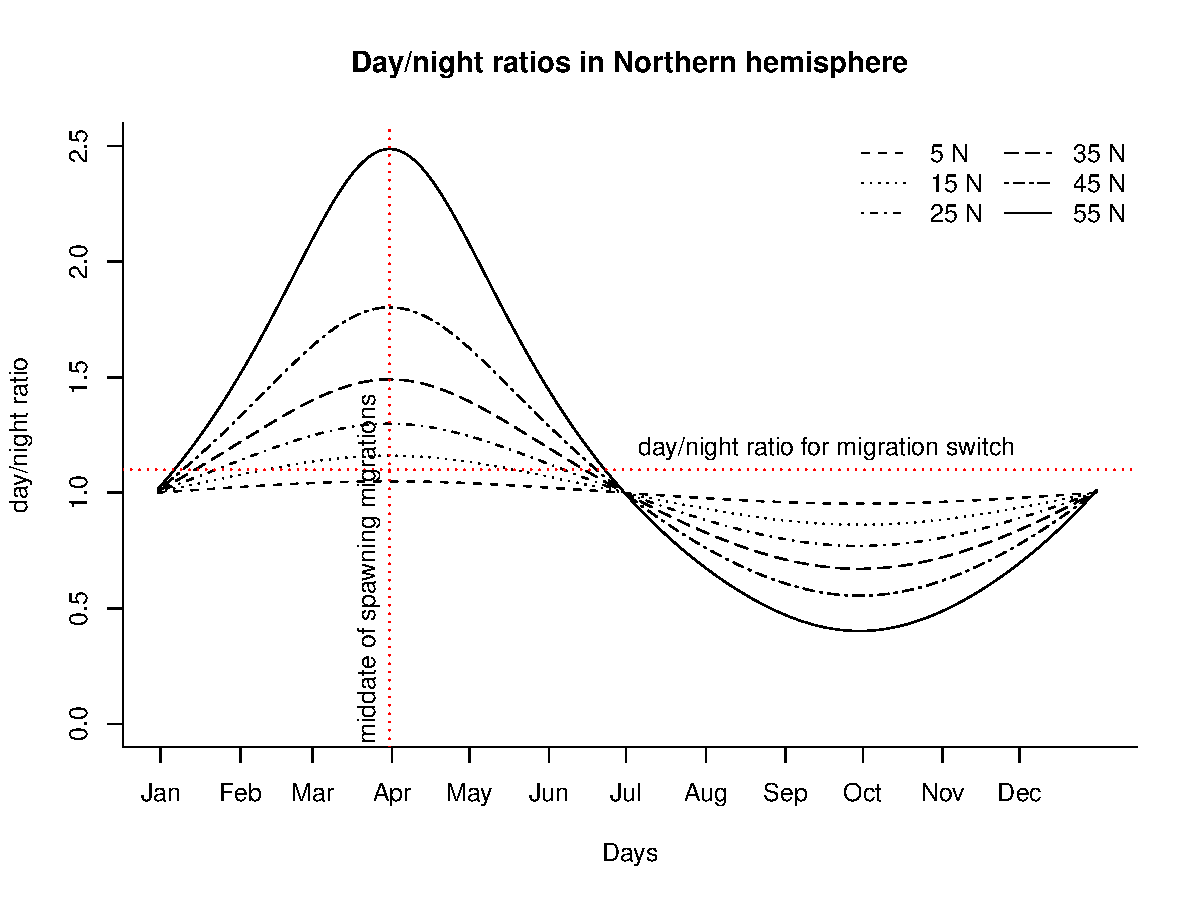
\includegraphics[width=0.75\textwidth]{chapter1/figs/DN-ratio}\\
  \includegraphics[width=0.75\textwidth]{chapter1/figs/seasonal_switch}
  \caption{Illustration of seasonal switch functions: (top) day-night ratio $\varrho$ for northern hemisphere; (bottom) the dates of seasonal switch eq.~\ref{eq:switch-function} between feeding and spawning migrations at different latitudes. The dotted vertical lines denote the mid-date, $\hat{t}$, of the spawning season. The parameter $\varrho_s$ defines the latitude, below which the seasonal switch does not occur. }
  \label{fig:seasonal-switch}
\end{figure}

However, the use of the switch function~\eqref{eq:switch-function} and the linear combination of feeding and spawning habitats~\eqref{eq:seasonal-habitat} may lead to two problems. First, the predefined seasonality of a daylight function does not necessarily align with the timing of albacore migrations to the spawning grounds. Second, when feeding and spawning habitats are characterised by very different oceanographic conditions, which is often the case for the temperate species (e.g. albacore, bluefin tuna), these two habitats, spawning and feeding, do not overlap geographically and hence there are no local cues that may stimulate long-distance migrations to spawning grounds. 

\paragraph{The flexible timing} of the spawning season is enabled by adding a time lag to the day $t^{\bigodot}$ of summer solstice:

\begin{equation}
\delta t=t^{\bigodot}-\hat{t},
\label{eq:season-peak}
\end{equation}

 
\noindent and computing the day length at day $t+\delta t$. So, for the day length $\lambda(t + \delta t,y)$, the $\hat{t}$ becomes the mid-date of the spawning season, also called a season peak. In this case the day length is used only as a convenient periodic function providing the seasonality at every latitude. Note that the choice of mathematical form of the function of day length, $\varrho$, should be done within the MLE approach given that parameters defining the moment of the switch $\varrho_s$, and the mid-date of the spawning season $\hat{t}$ can be effectively estimated from the data (Figure~\ref{fig:seasonal-switch-sigma}). For example, we can use the function of day length, the gradient of the day length, or the day-night ratio $\varrho=\lambda/(24-\lambda)$.


\begin{figure}[htbp]
  \centering
  \includegraphics[width=0.75\textwidth]{chapter1/figs/seasonal_with_sigma}
  \caption{Same as in figure~\ref{fig:seasonal-switch}, but including the variations of standard deviation of the Gaussian thermal function (dashed curve, right y-axis), enabling the local cues (expressed through non-zero gradients of seasonal habitat) for mature adult movements. Parameters of seasonal switch estimated based on fisheries data for south Pacific albacore \citep{Senina2020a}.}
  \label{fig:seasonal-switch-sigma}
\end{figure}

\paragraph{Local gradients} To enable the local cues and hence the non-zero velocities for tunas directed towards the spawning grounds and back to the feeding grounds, the following approach has been implemented. Based on the tuna sensitivity to water temperature and the hypothesis that adult tunas follow warmer temperatures while moving towards maturation and spawning areas \citep{LeGall}, we suggest using thermal gradients as the driver of migrations. In SEAPODYM, the temperature is the common environmental variable to which tunas respond within both feeding and spawning habitats. The thermal preferences at all ages $a \in (0,A^{+})$ are described by Gaussian-type functions with two parameters, ${T_a}^*$ and $\sigma_a$, being the preferred optimum and the temperature tolerance range respectively~\eqref{eq:feeding-thermal}. To link seasonal movements to thermal gradients, we assume that the range of preferred temperatures in the mature tuna’s habitat varies with time. It is maximal at the beginning of migrations, that is, at the moment of the switch, and decreases to the range of temperatures characteristic for the spawning at the seasonal peak. One way to describe this variable $\sigma_{a,s}(t)$ during the spawning season is to relate it linearly to the function of day length $\varrho(t,y_n)$ at a given (fixed to the northernmost) latitude $y_n$, namely to its deviation $\delta \varrho$ from its value at season peak $\varrho (\hat(t),y_n)$:

\begin{equation}
  \sigma_{a,s}=\sigma_0+\left(\bar{\sigma_a}-\sigma_0\right) \frac{\delta \varrho}{\delta \varrho_{max}} 
\label{eq:var-sigma}
\end{equation}

\noindent where $\sigma_0$ is the standard deviation providing a range of preferred temperatures in spawning habitat; $\bar{\sigma_a}={T_0}^*-{T_a}^*$ is the difference between optimal spawning temperatures and preferred temperatures of tunas aged $a$; and $\delta \varrho_{max}$ is the maximum deviation of the chosen day length functions. Note that one standard deviation $\sigma_{a,s}$ being the difference between $H_a$ and $H_s$ thermal optima provides the highest gradients of the Gaussian thermal function. The seasonality of the spawning migrations and variable thermal range $\sigma_{a,s}$ are illustrated in Figure~\ref{fig:seasonal-switch-sigma}. Note that the variability of $\sigma_{a,s}$ is effective only within a spawning season occurring once per year in each hemisphere. 



\subsection{Natural mortality}\label{sec:natural-mortality}

The natural mortality of fish includes two mechanisms --  population decay due to the predation process and population abundance decrease due to senescence of individuals with age, denoted $m_P(a)$ and  $m_S(a)$ , respectively. They are modelled in SEAPODYM by the following equations:

\begin{align}
	m_P(a) = \bar{m}_P e^{-\beta_P a} \label{eq:Mp}\\
	m_S(a)  = \bar{m}_S a^{\beta_S} \label{eq:Ms}
\end{align}
	
\noindent where parameter $\bar{m}_P>0$ is the maximal predation rate, corresponding to age 0 and $\bar{m}_S>0$ is the senescence mortality rate at $a=1$, and $\beta_P>0$ and $\beta_S>0$ define the rates of mortality change with age; their positiveness corresponds to an assumption that predation mortality decreases with age and senescence increases. So the total mortality rate is simply a sum of two terms, predation and senescence mortality (Figure~\ref{fig:mean-mortality}):

\begin{equation}
m(a) = m_P(a)+m_S(a)
\label{eq:M}
\end{equation}

\begin{figure}[htbp]
  \centering
  \includegraphics[width=0.55\textwidth]{chapter1/figs/mortality-func}
  \caption{Total mortality rates due to senescence,$m_S(a)$ eq.~\eqref{eq:Ms}, due to predation, $m_P(a)$ eq.~\eqref{eq:Mp}, the total mortality rate, $m(a)$ eq.~\eqref{eq:M}, as well as the range of variability of mortality rate $m_N$, eq.~(\ref{eq:Mvar}), related to feeding habitat index.}
  \label{fig:mean-mortality}
\end{figure}

In addition, it is assumed that at any age, the natural mortality can be altered by environmental conditions, such as temperature, availability of food and predators. Hence, we assume that total mortality rate $m$ can vary in space and time depending either on the spawning habitat index $H_s$ (for larval and small juvenile stages) or feeding habitat index $H_a$ for adult life stages. Let us denote $I$ the index of habitat occupied by the life stage:

%\begin{displaymath}
\begin{eqnarray}
 I = \left\{
 \begin{array}{cl}
	H_s\text{, if}& a=0\\
	H_j\text{, if}& a \in (0,a_J]  \\
	H_a\text{, if}& a>a_J
  \end{array} 
  \right.
\label{eq:H-in-M}  
\end{eqnarray}
%\end{displaymath}

\noindent where the index $H_j$, used to describe the conditions for survival of juveniles and affecting only the local (in every position $\mathbf{x}$) mortality rates of juveniles, is computed as follows:

\begin{itemize}
\item $H_j=f_1(\Lambda,\alpha) \times f_2(T_1;T^*_0,\sigma_0)$, or
\item same as above but including the density-dependent function accounting for cannibalism by adults. However, this is deliberately left out of the scope of this manual due to weak observability of the mechanism from fisheries data. 
\end{itemize}

\noindent It is important to note that index $H_j$ does not affect movements of juveniles, hence their distribution can be modified by $H_j$ only in case of strong environmental variability and the variable mortality effect estimated by the MLE approach (see chapter~\ref{ch:parametrisation}). 

To account for the effect of environmental conditions on local mortality rates, the mortality at age $m$ in eq.~\ref{eq:M} is affected by the habitat index variability in time and space. Hence the final formulation of a species' natural mortality $m_N=m_N(a,t,\mathbf{x})$ becomes:

	\begin{align}
	m_N & = m(a)(1+\varepsilon)^{1-2I}
	\label{eq:Mvar}
	\end{align}
	
\noindent where $\varepsilon$ is the parameter that gives the range of variability of mortality rate with habitat index within the range $m_N \in [m(a)/(1+\epsilon),m(a)(1+\epsilon)]$ where the minimal value corresponds to the most favourable habitat, $I=1$, and the maximal to the less favourable habitat, $I=0$. 


\subsection{Fishing mortality}\label{sec:FM}
In SEAPODYM, the mortality due to fishing $m_F=m_F(t,a,\mathbf{x})$ is computed based on two methods: 1) using  the Gordon--Schaefer formula and 2) using the catch removal method. The first classical approach relies on the geo-referenced observed fishing effort $E=E(t,\mathbf{x})$ as in the continuous Gordon--Schaefer model, and in the context of age explicit modelling, the mortality rate caused by fishing activity for the part of population at age $a$ is  

\begin{align}
&m_F(a)= q \cdot E \cdot s(a), 
\label{eq:Gordon--Schaefer}
\end{align}

\noindent where $q$ is the catchability of the fishing gear, and $s(a)$ is its selectivity for the fish at age $a$. Note, the fish population is usually harvested with different fishing gears, meaning that the model must consider multiple fisheries, so the catchability coefficient, $q_f$, fishing effort, $E_f$, as well as the gear selectivity, $s_f(a)$, are all fishery dependent. Then the total fishing mortality is computed as a sum of all mortality rates for fisheries being considered:

\begin{align}
&m_F(a)= \sum_f(q_f \cdot E_f \cdot s_f(a)). 
\label{eq:FM}
\end{align}

The selectivity, $s_f(a)$, being a function of age (length), is computed either as a non-linear concave function with a limit one (type I selectivity function), sigmoid function (type II selectivity function) or asymmetric Gaussian (type III):

\begin{eqnarray}
  \label{eq:fishery-specific-selectivity}
  s_{f}(a) = 
  \left\{\begin{array}{lll}
      \frac{\ell(a)}{\varsigma_f+\ell(a)},  & \textrm{  type I} \\
      \left(1+e^{-\varsigma_f (\ell(a)-\hat{l}_f)}\right)^{-1}, 
      & \textrm{  type II} \\
      e^{-\frac{(\ell(a)-\hat{l}_f)^2}{\sigma_{s_f}}}, 
      & \textrm{if $\ell(a)\leq\hat{l}$} \textrm{,  type II,}\\
      \mu_f+(1-\mu_f)e^{-\frac{(\ell(a)-\hat{l}_f)^2}{\sigma_{s_f}}}, 
      & \textrm{if $\ell(a)>\hat{l}$} \textrm{,  type III.} 
  \end{array}\right.
\end{eqnarray}	 


\noindent where
\begin{itemize}
\item $\varsigma_f$ is a half-saturation constant in the selectivity function type I;
\item $\varsigma_f$ is a slope coefficient in sigmoid-shape selectivity;
\item $\hat{l}_f$ and $\sigma_{s_f}$ are the parameters of Gaussian function (mean and standard deviation); and
\item $\mu_f$ is the asymptotic value of selectivity at large fish sizes.
\end{itemize}

\noindent The choice of the functional form of selectivity depends on fishing gear and hence is determined by different factors such as the use of hooks or seine, their depths and mesh size (in case of seine). For example, the sigmoid function is commonly used for long-line fishery, while for purse seine gear, operating at the surface and targeting mostly the younger (smaller) fish, type III is more appropriate (see Figure~\ref{fig:sq-plots}).  

\begin{figure}[htbp]
	\centering
		\includegraphics[width=1.00\textwidth]{chapter1/figs/plots_sq}
	\caption{Catchability and selectivity by fishery estimated for different optimization experiments for south Pacific albacore \citep*[from][]{Senina2020a}. The y-axis shows the product of catchability coefficient (constant in space and time) and selectivity function (varies with size between 0 and 1) so that the plot gives catchability by size. For fisheries for which a dashed line is present, the catchability was allowed to vary linearly in time to account for the change in the gears/strategy efficiency. In that case the dashed lines correspond to the catchability at size at the beginning of the run and the solid lines show the catchability at size at the end of the run.}
	\label{fig:sq-plots}
\end{figure}

The second method, called the \textit{catch removal} method, consists of subtraction of total (summarised over all fisheries) observed catch in number of fish of a given age class directly from the predicted fish density. Note that since catch is by definition a discrete variable, it is more convenient to use discrete notations for this variable as well as for all operators including it. Obviously, catch subtraction occurs only in those locations in space where catch is non-zero. Let us denote all variables in a position of a discretised space, that is, in a grid cell with indices $(i,j)$. 
Subscripts $f,K,p,i,j$ denote fishery, model integration time step index, age index and grid cell indices respectively (notations of Chapter 2~{\hypersetup{linkcolor=black}{\bfseries \nameref{ch:numerics}}}).

Let us denote by $N_{k,p,i,j}$ the population density in number of fish within age class $p$ per unit area at the model integration sub-step $k\frac{\Delta T}{n_t}$ ($k=1,\dots,n_t$, $n_t$ -- number of iterations in the inner loop of ADI method). Quantity $C^{\text{obs}}_{k,p,i,j}=\frac{1}{n_t}C^{\text{obs}}_{K,p,i,j}$ is the $n$th portion of the total observed catch in number of individuals from age class $p$ and time interval $K$. The fishing mortality is accounted through the subtraction (removal) of the observed catch directly from the population density at the ADI method sub-step. To ensure the positivity of the fish population density, it can only be reduced by the amount that corresponds to the sustained catch, that is smaller than the model biomass in a given position in space. Hence, we have the following:

\begin{align}
&N_{k+1,p,i,j} = N_{k,p,i,j}-\text{min}\left(\frac{C_{k,p,i,j}^{\text{obs}}}{\Delta x_i \Delta y}, N_{k,p,i,j}\right),
\label{eq:MCR}
\end{align}

\noindent where a differentiable version of the min function is implemented using a rotated hyperbola in order to avoid a problem of the non-differentiability of the minimum of two values.

Note that the age stratification in catch is usually not available in the observational datasets, but the fraction of observed total catch by age $C_{p,i,j}^{\text{obs}}$ can be derived either from the observed length frequency distributions, or simply using the model fishery selectivity function. Because of scarcity of fine-resolution length frequency data, currently the second method is implemented. The latter means that in the catch removal method even though we use the observed quantities, the mortality induced by a fishery depends on model parameters. For more details on catch prediction and parameter estimation see chapter 4~{\hypersetup{linkcolor=black}{\bfseries \nameref{ch:parametrisation}}}.


\begin{comment}
%\section{Model predictions}\label{sec:model-predictions}
%
%%\subsection{Population biomass}\label{sec:predicted-biomass}
%
%\subsection{Catch}\label{sec:predicted-catch}
%In the current version there are two methods of computing fishing mortality and predicted catch: 1) using Gordon--Schaefer formula and 2) using catch removal method. See the fishing mortality methods in section~\ref{sec:FM} in chapter~\ref{ch:model}. The first method is based on the fishing effort. The mortality due to fishing $F_{fa}$, computed in eq.~\ref{FM}, depends on the catchability, $q_f$, of the fishing gear $f$, its selectivity, $s_{fa}$, for the fish at age $a$, and the observed fishing effort, $E_{f}$. The predicted catch $C^{\text{pred}}$ is then computed based on the geo-referenced observed fishing effort $E$ as follows: 
%
%\begin{align}
%&C^{\text{pred}}_{fatij} = F_{fatij} \cdot N_{atij} \cdot \Delta x_i \Delta y_j 
%\label{eq:GS-catch-prediction}
%\end{align}
%
%where sub-scripts $fatij$ denote fishery, age, time step and grid cell indices respectively; $N_{atij}$ is the abundance of fish and $C^{\text{pred}}_{fatij}$ is the total predicted catch in numbers of fish of age $a$. The total predicted catch of fishery $f$ at time $t$, $C^{pred}_{tfij}$ and in weight of fish, is then computed in the model using observed fishing effort $E_{tfij}$ at location $(i,j)$ by 
%
%\begin{align}
%C^{pred}_{tfij}=q_f E_{tfij} \sum\limits^K_{a=1} s_{fa} w_a N_{aij} \mathit{\scriptstyle\Delta} x \mathit{\scriptstyle\Delta} y,
%\label{eq:catch-in-weight}
%\end{align}
%
%
%\noindent where $w_a$ is the mean weight of fish in the $a$-th cohort.
%
%Thus, predicted catch depends not only on the available fish biomass, but equally depends on the fishing effort, gear catchability and selectivity. In SEAPODYM the selectivity parameters do not vary in space and time and catchability is either constant or allowed to change linearly over time. Therefore, the estimation of population spatial distribution in the MLE approach is essentially driven by the spatio-temporal variations of the biomass and the fishing effort. 
%
%Such approach is correct only in the ideal case, i.e. when the fishing effort is well estimated and fully reported. For gears such as purse-seine the estimation of fishing effort is problematic as one should take into account not only the number of sets which were employed after the fish school has been detected, but also the time the boat spent for active searching. The second variable is often hard to estimate and usually the effort becomes inflated in the principal fishing grounds characterized as zones with highest catches and where the fishing boats spend more time and underestimated in the areas, which are rarely visited by the fishermen. As an example, the observed catch per unit of effort (CPUE) of purse-seine fisheries targeting free schools of skipjack are higher outside of main fishing grounds thus showing a clear density gradient towards their edges. 
%
%To avoid the biases associated with the use of inaccurate fishing effort, another method was implemented (see chapter~\ref{ch:parametrisation} for more details). It consists in removal of total (summarized over all fisheries) catch in number of fish of a given age class directly from the predicted fish density. Let us denote $N_{akij}$ - the population density in number of fish of age $a$ per unit area at the model integration step (inner loop in chapter~\ref{ch:numerics}), $k\frac{\Delta t}{n}$ ($k=1..n$, $n$ - number of iterations in ADI method); $C^{\text{obs}}_{akij}=\frac{1}{n}C^{\text{obs}}_{atij}$ is the n-th portion of the total observed catch at time $t$. Then the corresponding predicted catch at the ADI method sub-step is computed as follows:
%
%
%\begin{align}
%&C^{\text{pred}}_{akij} = \text{min}\left(C_{akij}^{\text{obs}}, (N_{akij} \cdot \Delta x_i \Delta y_j) \right).
%\label{eq:catch-removal}
%\end{align}
%
%
%Note, that according to the eq.~\ref{eq:catch-removal} the predicted catch is either equal or less than the observed one. The later happens only if there is not enough biomass in the grid cell. Finally the predicted total catch is attributed to the fisheries $f$ operating in the cell $ij$ according to their observed ratio, i.e.
%
%\begin{align*}
%C^{\text{pred}}_{fatij} = \frac{C^{\text{obs}}_{fatij}}{\sum_f C^{\text{obs}}_{fatij}} \sum_{k=1}^N C^{\text{pred}}_{akij}
%\label{eq:CR-catch-at-age}
%\end{align*}. 
%
%The use of Eqs.\ref{eq:CR} and \ref{eq:MCR} can be combined with the classical approach~\eqref{eq:FM} by applying the later to selected fisheries, for which the fishing effort can be considered unbiased (long-line and pole-and-line fisheries targeting modelled species). One inconvenience of the catch removal approach is that it cannot combine catch data with different units (e.g., metric tons and numbers of fish).  
%
%
%\subsection{Length frequency}\label{sec:length-frequency}
%
%The length frequency, in other words, the predicted proportion at age $a$ in the catch at time $t$ for fishery $f$ in region $r$ is
%
%  \[ Q^{pred}_{tfar}=\frac{s_{fa} \sum\limits_{i,j \in r} E_{fij} N_{aij}\mathit{\scriptstyle\Delta} x \mathit{\scriptstyle\Delta} y}{\sum\limits^K_{a=1} s_{fa} \left(\sum\limits_{i,j \in r} E_{fij} N_{aij}\mathit{\scriptstyle\Delta} x \mathit{\scriptstyle\Delta} y\right)}
%\]
%
%\noindent where indices $ij \in r$, with region $r$ defined by observations, which are usually given at coarser than model resolution (from $5^{\circ} \times 5^{\circ}$ to $10^{\circ} \times 20^{\circ}$); $\Delta x$ and $\Delta y$ are the spatial resolution of computational grid (see~\ref{ch:numerics} for more details). 

\end{comment}

\section{Model parameters}\label{sec:parameters}
We summarise in Table~\ref{tab:parameters} all model parameters that control the SEAPODYM dynamic processes described in this chapter. Note that biological parameters that are used to compute species' length-at-age, weight-at-age as well as maturity-at-age (section~\ref{sec:sp-biology}), are not included in this table as they are not SEAPODYM parameters and usually estimated in external studies. As described in section~\ref{sec:model-dyn}, all dynamic processes in the model are linked to the environmental variables. In addition, the spatial dynamics (movement) that greatly influences all demographic processes in heterogeneous environments, is modelled explicitly. Therefore, a complex and highly dimensional dynamics can be governed by a limited number of parameters. They are listed in Table~\ref{tab:parameters}: reproduction parameters controlling spawning habitat, $H_s$, and source term, $S$; five parameters of natural mortality, $M$; 12 parameters for feeding habitat, $H_a$; and four parameters of movement rates, among which two control advection rates $v_N$ and two define diffusion rates, $D$. In addition, there are two to four parameters per fishery, which contribute to model dynamics through fishing pressure, the number of them depending on the use of a mortality equation (\ref{eq:FM} or \ref{eq:MCR}) and selectivity function eq.~\ref{eq:fishery-specific-selectivity}. However, fisheries parameters also influence  the model predictions, such as predicted catch-at-age and length frequency of catch. The methods for catch and length frequency data predictions are fully detailed in Chapter~\ref{ch:parametrisation}. 

\begin{longtable}{p{.75cm}p{1.5cm}p{11cm}p{1.5cm}}
\caption{Species dynamic parameters with their notations, definitions and  references\label{tab:parameters}}\\\hline
$\boldsymbol \uptheta$	& \textbf{Eq.}&  \textbf{Description} & \textbf{Units}	\\\hline 
\endfirsthead
%\multicolumn{3}{@{}l}{\ldots continued}\\\hline
\multicolumn{3}{@{}l}{Table 1.3 continued}\\\hline
$\boldsymbol \uptheta$	& \textbf{Eq.}&  \textbf{Description} & \textbf{Units}	\\\hline 
\endhead % all the lines above this will be repeated on every page
\hline
%\multicolumn{3}{r@{}}{continued \ldots}\\
\endfoot
\hline
\endlastfoot
    \multicolumn{4}{c}{\textit{Recruitment}} \\
\hline
    $r$ &(\ref{eq:larvae})  &{Reproduction rate in Beverton--Holt function}&$\text{mo}^{-1}$\\
    $b$ &(\ref{eq:larvae})  & {slope parameter in Beverton--Holt function}&$\text{Nb}^{-1}\text{km}^2$\\\hline
    \multicolumn{4}{c}{\textit{Natural mortality}}\\
\hline
    $\bar{m}_p$ &(\ref{eq:Mp}) & {Predation mortality rate age age $0$}&$\text{mo}^{-1}$\\

    $\beta_p$&(\ref{eq:Mp})& {Slope coefficient in predation mortality} &\\

    $\bar{m}_s$ & (\ref{eq:Ms}) & {Senescence mortality rate at age $0$}&$\text{mo}^{-1-\beta_s}$\\

    $\beta_s$ &(\ref{eq:Ms})   & Slope coefficient in senescence mortality&\\

    $\epsilon$ &(\ref{eq:Mvar}) & {Variability of mortality rate with habitat index from $\frac{M}{(1+\epsilon)}$ in the worst habitat to $M(1+\epsilon))$ in the best habitat} &\\\hline

   \multicolumn{4}{c}{\textit{ Spawning habitat}} \\
\hline
    $\sigma$ &\eqref{eq:spawning-thermal}  & {Standard deviation in temperature Gaussian function of spawning habitat}&$^\circ \text{C}$\\

    $T^{\star}$ & \eqref{eq:spawning-thermal} &{Optimal surface temperature for larvae in spawning habitat definition}&$^\circ \text{C}$\\

    $\alpha$ &\eqref{eq:spawning-prey} & {Prey encounter rate in Holling (type III) function} &$\text{day}^{-1}$\\
    $\alpha_{F}$ &(\ref{eq:spawning-pred})  & Log-normal mean parameter in predator-dependent function & g$\cdot$m$^{-2}$\\
    $\beta_{F}$ &(\ref{eq:spawning-pred})  & Log-normal shape parameter in predator-dependent function &\\
\hline
   \multicolumn{4}{c}{\textit{ Feeding habitat}}\\
\hline   
    $T_0$ & (\ref{eq:temperature-length})& {Preferred temperature for age 0} &$^\circ \text{C}$\\
    $T_m$ & (\ref{eq:temperature-length}) & {Preferred temperature for the oldest adult fish} & $^\circ \text{C}$\\ 
    $\sigma_0$ & (\ref{eq:sigma-weight}) 	 & Standard deviation in temperature Gaussian function for age 0 in feeding habitat& $^\circ \text{C}$\\ 
    $\sigma_m$ & (\ref{eq:sigma-weight}) 	 & Standard deviation in temperature Gaussian function at age A+ &  $^\circ \text{C}$\\       
    $b_T$ &(\ref{eq:temperature-length})& {Allometric power coefficient for thermal preferences at age} &\\
    $\gamma$ &(\ref{eq:oxygen})  & {Slope of the oxygen function in layer accessibility}&\\

    $\hat{O}_2$ &(\ref{eq:oxygen}) 	& {Critical value of dissolved oxygen in the layer}& ml/L\\
    
    $E_{11}$ &(\ref{eq:eF-matrix})& Epipelagic forage scaling factor & m$^2\cdot$g$^{-1}$\\
    $E_{22}$ &(\ref{eq:eF-matrix})& Mesopelagic forage scaling factor & m$^2\cdot$g$^{-1}$\\
    $E_{21}$ &(\ref{eq:eF-matrix})& Migrant mesopelagic forage scaling factor & m$^2\cdot$g$^{-1}$\\
    $E_{33}$ &(\ref{eq:eF-matrix})& Lower mesopelagic forage scaling factor & m$^2\cdot$g$^{-1}$\\
    $E_{32}$ &(\ref{eq:eF-matrix})& Migrant lower mesopelagic forage scaling factor & m$^2\cdot$g$^{-1}$\\
    $E_{31}$ &(\ref{eq:eF-matrix})& Highly migrant lower mesopelagic forage scaling factor & m$^2\cdot$g$^{-1}$\\
\hline
    \multicolumn{4}{c}{\textit{ Adult seasonal migrations}} \\
\hline
    $\hat{t}$ &(\ref{eq:switch-function}) & Mid-date (day of the year) of seasonal spawning migrations of adults &\text{day}\\
    
    $\varrho_s$ &(\ref{eq:season-peak}) & Critical value of day-night ratio, $\varrho$, triggering seasonal migrations& \\
\hline
  \multicolumn{4}{c}{\textit{ Movement}} \\
\hline
    $c$ &\eqref{eq:diffusion} & {Coefficient of diffusion variability with habitat index}&\\
    $\sigma$ &\eqref{eq:diffusion}& {Multiplier for the theoretical diffusion rate $\frac{{\bar{V}}^2 \Delta T}{4}$}& \\
    $V_m$ &\eqref{eq:taxis-coefficient} & {Velocity at maximal habitat gradient and $A=1$, $\text{BL}/\text{s}$}& \\
    $A$ &\eqref{eq:taxis-coefficient} &{Slope coefficient in allometric function for tuna velocity}&\\
\hline
     \multicolumn{4}{c}{\textit{ Fishing mortality and catch prediction}} \\
\hline
    $q_f$ &(\ref{eq:FM},~\ref{eq:catch-in-weight})   & Constant catchability coefficients for all declared fisheries&\\
    $\varsigma_f$ &(\ref{eq:fishery-specific-selectivity})  & Steepness of selectivity function if type I or II, standard deviation if type III&$\text{cm}$\\
    $\hat{l}_f$ & (\ref{eq:fishery-specific-selectivity})  & Threshold length in sigmoid function; mean length in asymmetric Gaussian function &$\text{cm}$ \\
    $\mu_f$ &(\ref{eq:fishery-specific-selectivity}) & Lowest selectivity for large fish in case of asymmetric Gaussian selectivity function&\\		
\hline        
\end{longtable}


\addcontentsline{toc}{section}{References}


\begin{thebibliography}{}

\bibitem[Lehodey et al., 1998]{Lehodey1998} Lehodey P., André J-M., Bertignac M., Hampton J., Stoens A. 1998. Predicting skipjack tuna forage distributions in the Equatorial Pacific using a coupled dynamical bio-geochemical model. \textit {Fisheries Oceanography} 7: 317–325.

\bibitem[Lehodey et al., 2010]{Lehodey2010} Lehodey, P.,  Murtugudde R., Senina I. 2010. Bridging the gap from ocean models to population dynamics of large marine predators: A model of mid-trophic functional groups. \textit{Progress in Oceanography}, Volume 84:69-84.

\bibitem[Lehodey et al., 2015]{Lehodey2015} Lehodey P., Conchon A., Senina I., Domokos R., Calmettes B. et al. 2015. Optimization of a micronekton model with acoustic data. ICES Journal of Marine Research. 53, 571-607. Science 72(5):1399–1412. \url{https:/doi.org/10.1093/icesjms/fsu233}

\end{thebibliography}

